\chapter{Introducción}

Los comentarios en videos en vivo son parte importante de la respuesta de la audiencia y se entiende que estos comentarios este cargados de palabras emotivas o que representen los sentimientos que las personas intentan comunicar al resto de espectadores, incluso a los mismos creadores del contenido o participantes de la transmisión en vivo, por lo que es de esperar que estos se expresen de forma positiva o negativa, de igual forma estos comentarios pueden ser poco objetivos, claramente objetivos o muy subjetivos.\\

El análisis de sentimientos implica el procesamiento del lenguaje natural de modo que se logre identificar información subjetiva de un texto en particular, en esta tarea buscamos identificar el sentimiento subjetivo expresado por los usuarios que dejaron un comentario en la transmisión en vivo del primer debate presidencial \cite{quiroga2016}.\\

\section{Objetivos}
El objetivo de este trabajo es identificar el sentimiento expresado por los usuarios en los comentarios del debate, teniendo en cuenta los votos que recibieron los comentarios y el sentimiento presente en los comentarios mas botados, al igual que la respuesta general de los sentimientos de la audiencia.\\ 

\begin{enumerate}
	\item Identificar la polaridad de los comentarios que la audiencia dejo en el video del debate.\\
	
	\item Identificar el nivel de objetividad y subjetividad de los comentarios en el video.\\
	
\end{enumerate}

\chapter{Análisis de sentimiento}

\cite{quiroga2016}, considerando lo siguiente:

\begin{itemize}
	\item Se consideran con polaridad muy negativa los comentarios 
	\begin{itemize}
		\item $0> y \geq-1 $
	\end{itemize}
	\item Se consideran con polaridad neutral los comentarios 
	\begin{itemize}
		\item $= 0 $
	\end{itemize}
		\item Se consideran con polaridad muy positiva los comentarios 
	\begin{itemize}
		\item $0< y  \geq 1 $
	\end{itemize}
\end{itemize}



\chapter{Procesado de los comentarios}

\begin{figure}[!h]
	\centering
	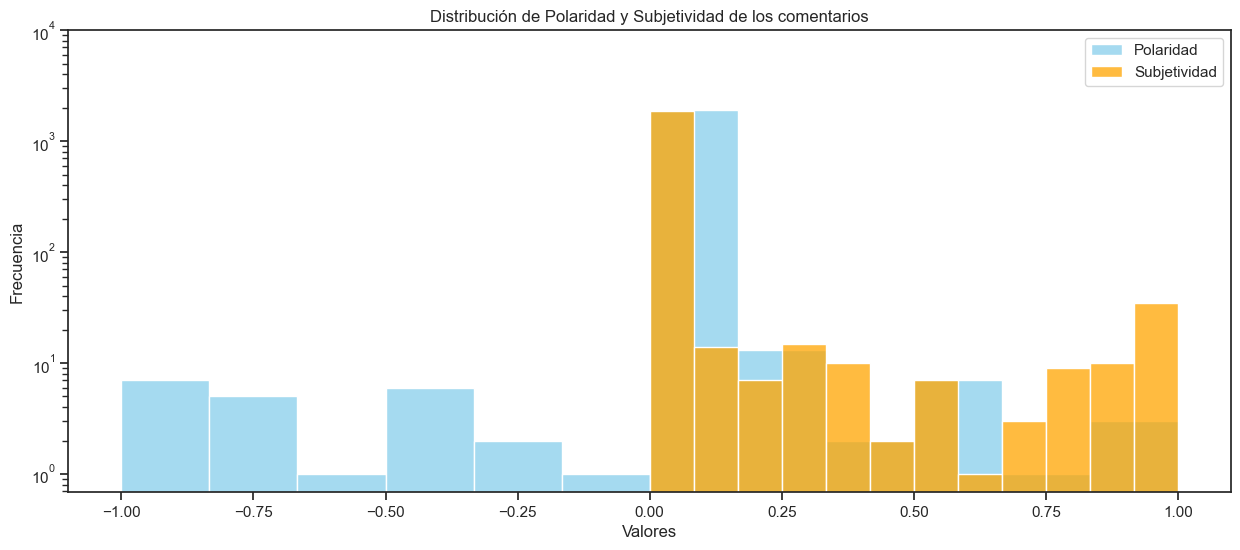
\includegraphics[width=16cm]{../Datos/polaridadYsubjetividad}
	\caption[Distribución de polaridad y subjetividad]{Distribución de la polaridad y subjetividad de los comentarios del primer debata presidencial.}
	\label{fig:dpys}
\end{figure}


\begin{figure}[!h]
	\centering
	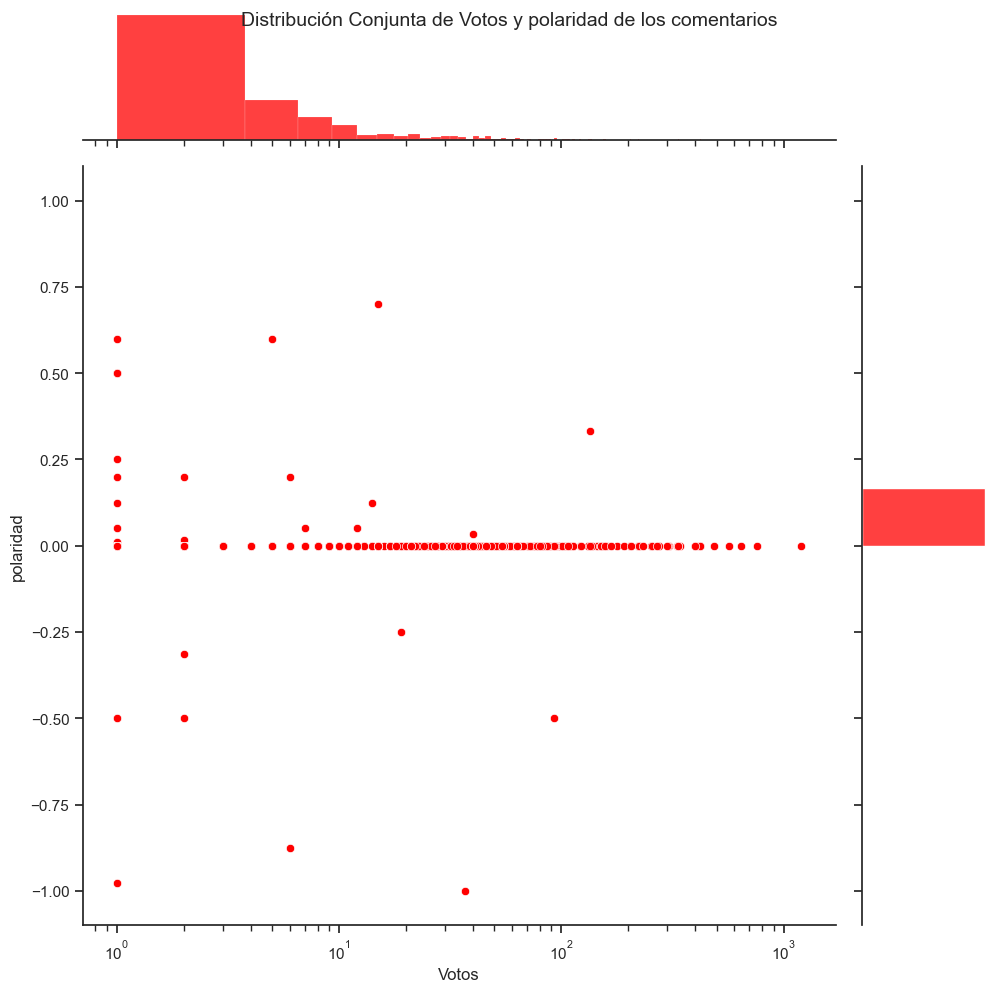
\includegraphics[width=16cm]{../Datos/DisVotosPolaridad}
	\caption[Distribución de frecuencia de voto y su polaridad]{Distribución de votos y la polaridad asociada con el interés y aprobación del publico.}
	\label{fig:dvp}
\end{figure}


\begin{figure}[!h]
	\centering
	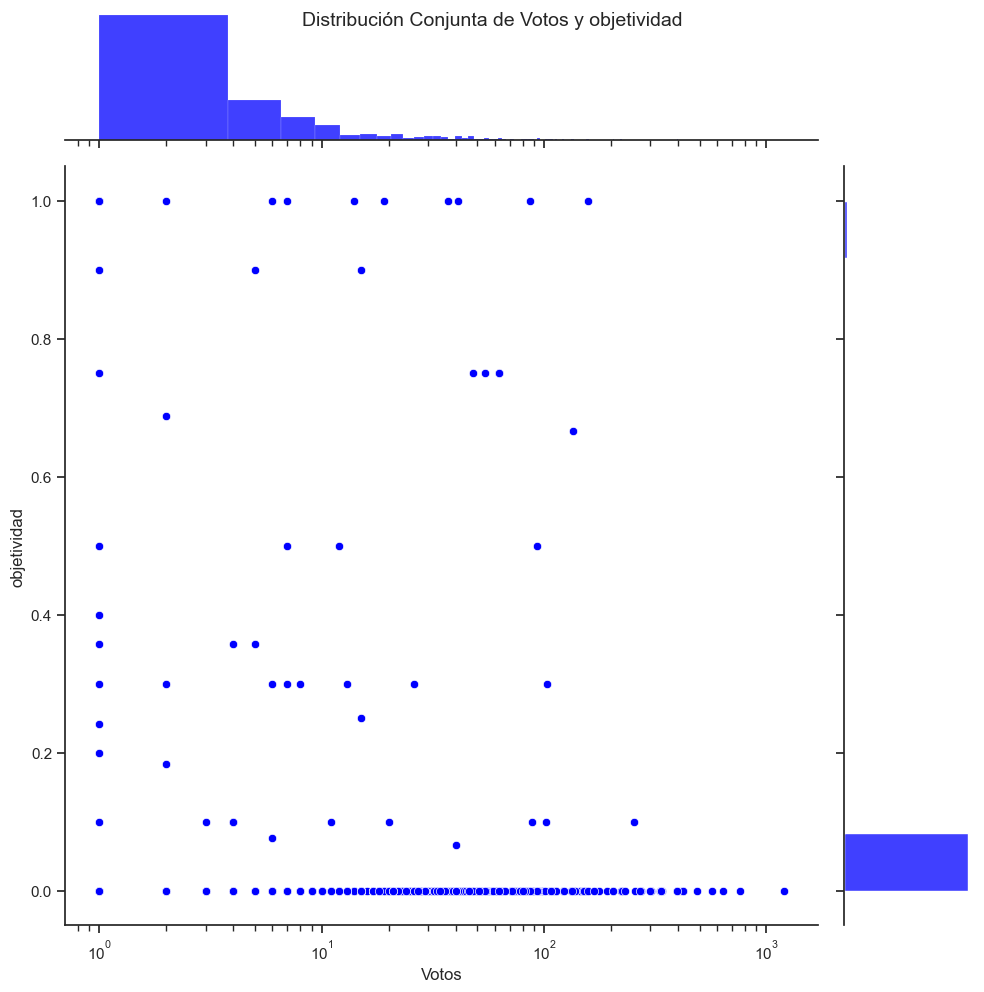
\includegraphics[width=16cm]{../Datos/DisVotosObjetividad}
	\caption[Distribución de frecuencia de voto y objetividad]{Distribución de la frecuencia de los votos y la objetividad de los comentarios}
	\label{fig:dvo}
\end{figure}


\chapter{Conclusiones}

